\appendix
\titleformat{\chapter}[block]{\normalfont\LARGE\bfseries}{Appendix \thechapter \;\textendash\;}{0ex}{\vspace{-4cm}}[\vspace{4.5cm}]
\titlespacing{\chapter}{0cm}{0cm}{0cm}

\chapter{Various Parameters}
\label{chap:appendix}

\begin{figure}[H]
  \centering
  \label{fig:bump-solutions}
  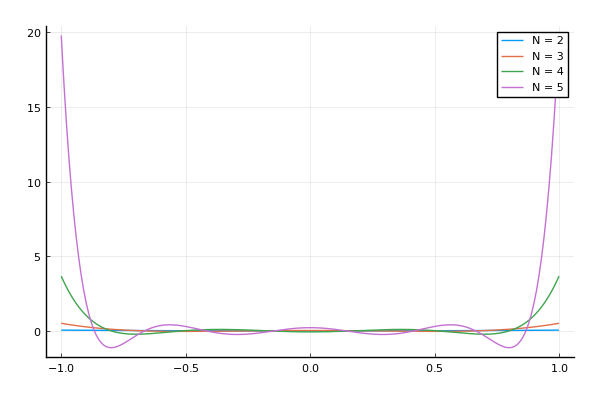
\includegraphics[width=0.6\linewidth]{results/bump/solution-increasing-order}
  \caption[Bump parameter solutions]{Solutions with bump parameters.}
\end{figure}

\begin{figure}[H]
  \centering
  \label{fig:spatial-energy-dependence}
  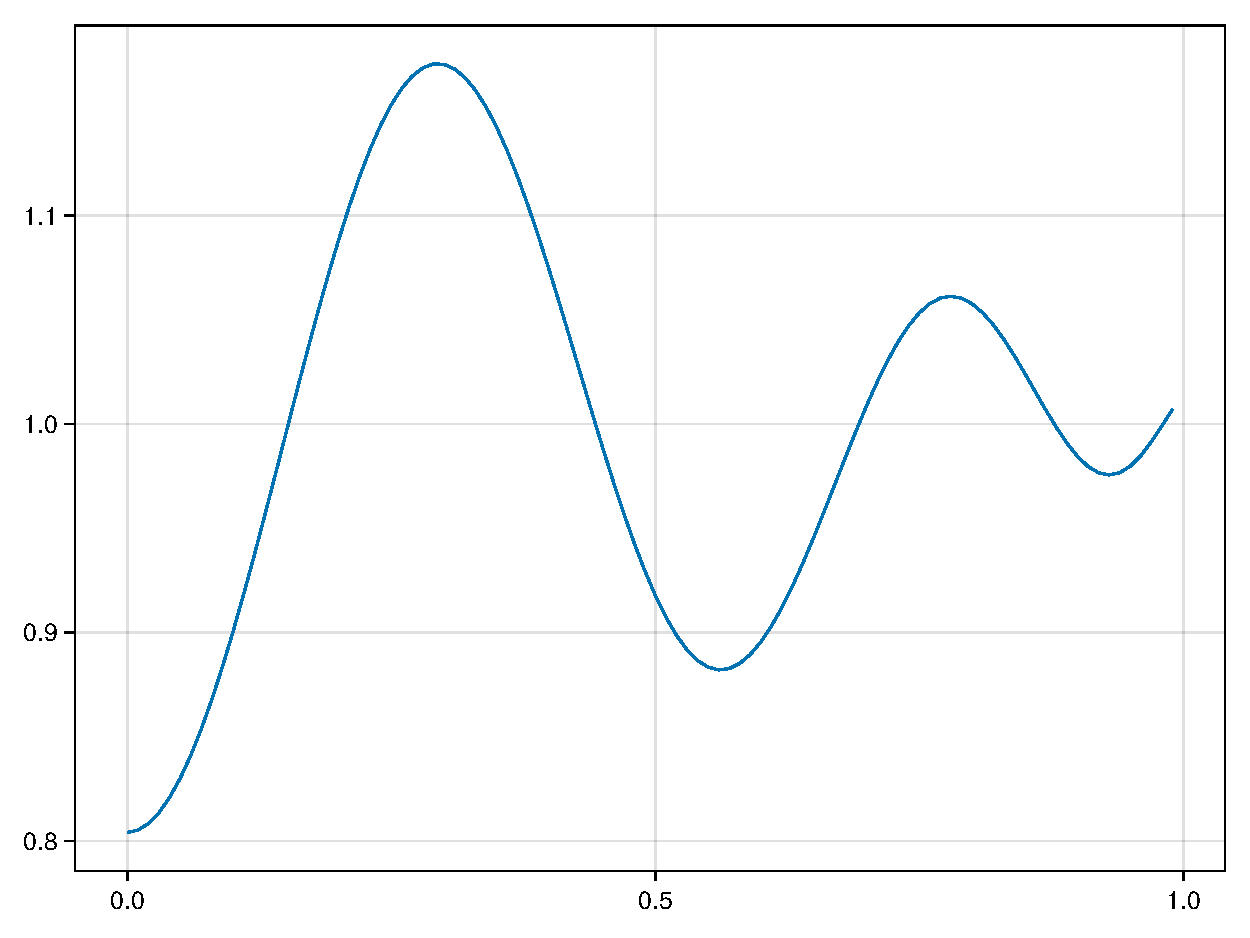
\includegraphics[width=0.7\linewidth]{results/attrep/energy-dependence-on-r.pdf}
  \caption[Spatial energy dependence on $r$]{Plot of the spatial energy dependence on $r$, for different values of the domain support radius $R$. As one can see, $E(\vec{x}) = \jacobivec{x} Q_{\alpha,\beta} \vec{\rho}$ constant and this figure is only present as visual proof to increase our confidence in the construction of the spectral method.}
\end{figure}

% \chapter{Supplemental Proofs}
